\vspace*{\fill}
\section{Infusing deep neural networks with physics}
\label{sec:lolaintro}
\begin{centering}
\textit{
The previous chapter ended by mentioning two ingredients that will become important for future searches with the multi-dimensional fit: A better vector boson tagger, and a generic anti-QCD tagger for signal independent searches. As a side project during my final PhD semester, I worked on a solution for the first, which has the added benefit of being a stepping stone towards the latter. This is what I will cover in the final chapter of this thesis.
\newline
\newline
When applying machine learning to particle physics problems, the input has historically consisted of pre-computed high-level features (quantities based on lower-level variables and certain theoretical assumptions).
With the rise of deep learning however, computational graphs have achieved an increased capability to find even the smallest correlations in datasets, allowing them to construct complex features on their own. The deep neural network (DNN) I will present in the following is based on the assumption that, given sufficient instructions about the laws of Nature, a neural network should be capable of reconstructing its own high-level features based on lower-level variables only. In addition, if smartly designed, the network should be capable of finding novel correlations and physical features, a-priori unknown, by allocating a physical meaning to the training weights deep within the network. The deep neural network I will present here, is trained to discriminate quark/gluon jets from W-jets. However, as I will discuss in the final section of this chapter, it is also the perfect starting point for developing a generic anti-QCD tagger.
\newline
\newline
The work presented in the following has not been published and still qualifies as work in progress. However, I believe developing taggers such as these is of great importance for future versions of the searches presented here, and is something I hope to continue working on in the future..
}
\begin{figure}[b!] 
    \centering
    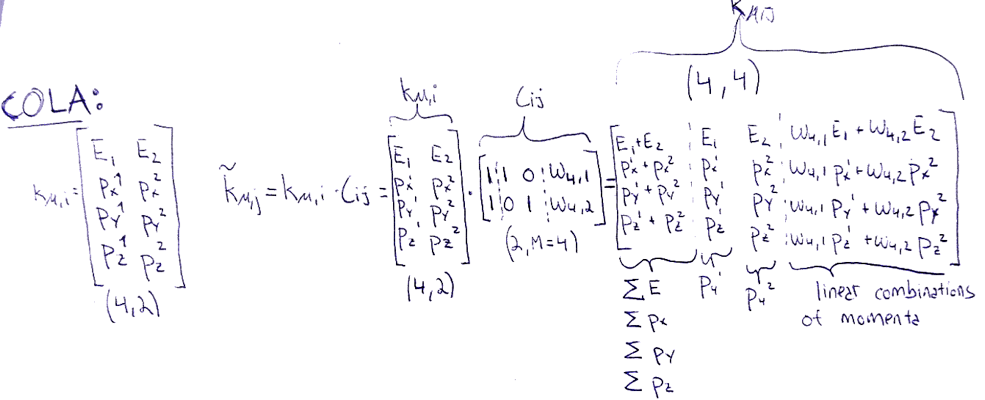
\includegraphics[width=10cm]{figures/vtagging/misc/cola.png}
    \vspace*{10mm}
    \caption*{\footnotesize{\textit{ ``What can we teach the machine?'' $\rightarrow$``What can we learn from the machine?'' Work in progress}}}
\end{figure}
\end{centering}
\clearpage
\vspace*{\fill}

\section{LoLa}
LoLa is a deep neural network architecture which was first introduced for top tagging~\cite{Butter:2017cot}. It is based on the idea that, given enough information about the laws of Nature, a neural network should be capable of calculating jet substructure observables on its own given only low-level information. The network is designed to discriminate between AK R=0.8 jets originating from W bosons from those originating from quarks or gluons, solely based on the jet constituent four-vectors (variables with little discriminating power on their own) as illustrated in Figure~\ref{fig:lola:4vec}.
\begin{figure}[h!]
\centering
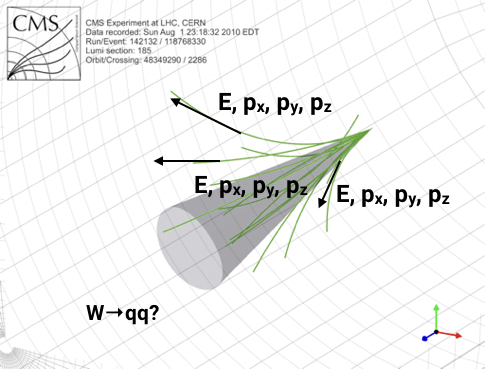
\includegraphics[width=0.33\textwidth]{figures/vtagging/misc/4vec.png}
\caption{LoLa uses only jet constituent four-vectors as input to discriminate W from q/g jets.}
\label{fig:lola:4vec}
\end{figure}
Rather than being fed high-level features, the neural network is given tools to perform calculations on Lorentz vectors using the Minkowski metric. Through two novel layers, linear combinations similar to jet clustering and jet substructure algorithms are performed, allowing the algorithm to create its own substructure variables. Additionally, training weights deep within the network correspond to physical quantities reconstructed by the algorithm; distance between particles, masses and energies, linear combinations of particle four-vectors etc.
Besides the end goal of discriminating Ws from quarks and gluons, one could therefore hope to learn of new correlations separating QCD from vector boson jets.

\subsection{Architecture}
The LoLa architecture is designed as a four layer deep, feed-forward sequential network doing supervised learning on fixed size input vectors.
Two novel layers are introduced, the Combination Layer (CoLa) and the Lorentz Layer (LoLa), which perform basic jet clustering and substructure calculations as well as implements the Minkowski metric.
These two layers are then followed by two fully connected layers, consisting of 100 and 50 nodes respectively, before the final output is computed using a Softmax activation function, yielding output probabilities between 0 and 1. The loss function to be minimized is "categorical crossentropy" (or log loss) where the two categories in use are W versus non-W probabilities. Only the W jet probability is stored.
The optimizer used in the training is the, now "standard", ADAM optimizer, which adapts the learning rate of the model parameters during training. The code itself is written using the Keras interface with a TensorFlow backend.
The full architecture with input and output dimension per layer is shown in Figure~\ref{fig:lola:arch}. The three first boxes are matrices, while the final four boxes correspond to vectors of different length. In the following, each layer will be explained in detail.
\begin{figure}[h!]
\centering
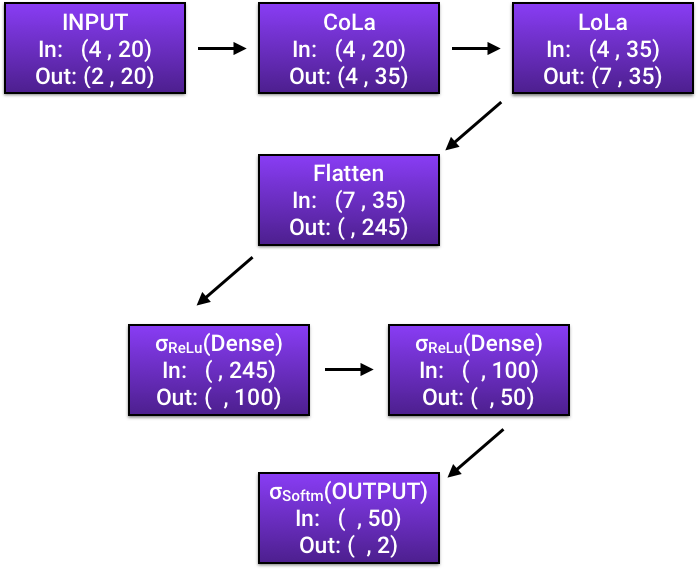
\includegraphics[width=0.59\textwidth]{figures/vtagging/misc/architecture.png}
\caption{The full LoLa architecture. ``In'' denotes the dimension of the input tensor to the given layer, ``Out'' is the output tensors dimensions.}
\label{fig:lola:arch}
\end{figure}


\subsection{Input}
This algorithm is trained to discriminate between fully merged hadronic W-jets coming from the process $\BulkG \rightarrow WW \rightarrow q\bar{q}q\bar{q}$ (where $M_{\BulkG}=0.6-4.5\TeV$), and quark/gluon jets from a QCD sample generated with \PYTHIA{8}Pythia 8. All jets are clustered with the anti-\kt algorithm with a distance parameter of R=0.8, with the PUPPI pileup removal algorithm applied. In addition, they are required to have $\PT > 200 \GeV$ and $|\eta| < 2.5$. 
Jets are defined as W-jets if they are matched to a generator level hadronically decaying W bosons, with the following matching criteria:
The generated vector boson needs to be within $\Delta R < 0.6$ of the jet axis, and the quark decay products need to be within $\Delta R < 0.8$ of the jet axis. The \PT and $\eta$ distribution of signal and background jets, is shown in Figure~\ref{fig:lola:kinematics}.
\begin{figure}[h!]
\centering
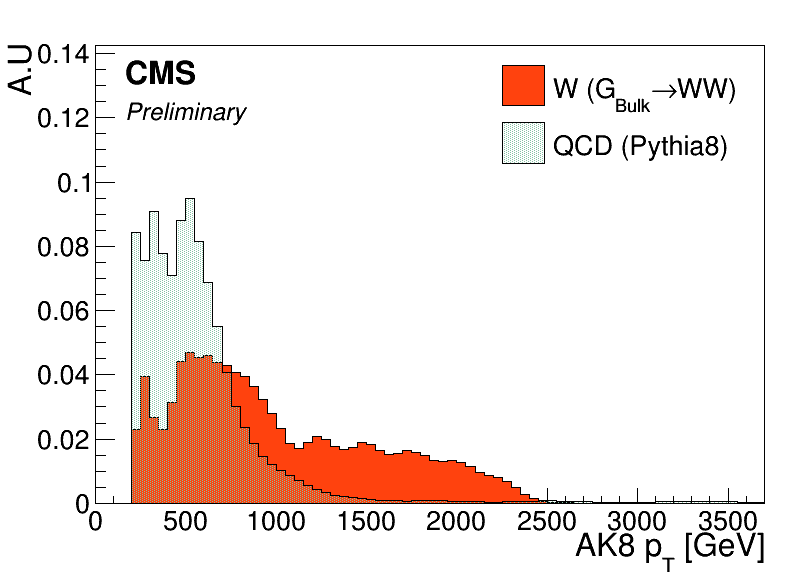
\includegraphics[width=0.49\textwidth]{figures/vtagging/AN-18-099/input/inputs/sig-bkg/jpt.png}
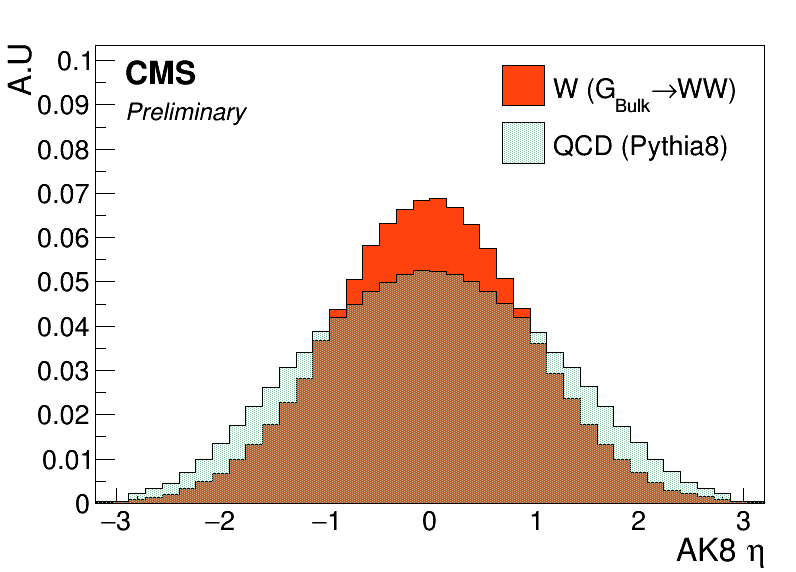
\includegraphics[width=0.49\textwidth]{figures/vtagging/AN-18-099/input/inputs/sig-bkg/jeta.png}\\
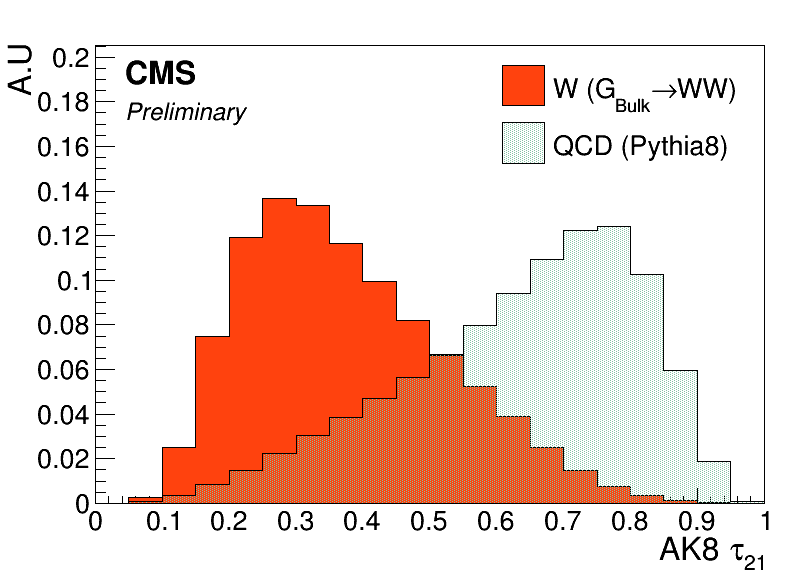
\includegraphics[width=0.49\textwidth]{figures/vtagging/AN-18-099/input/inputs/sig-bkg/jtau21.png}
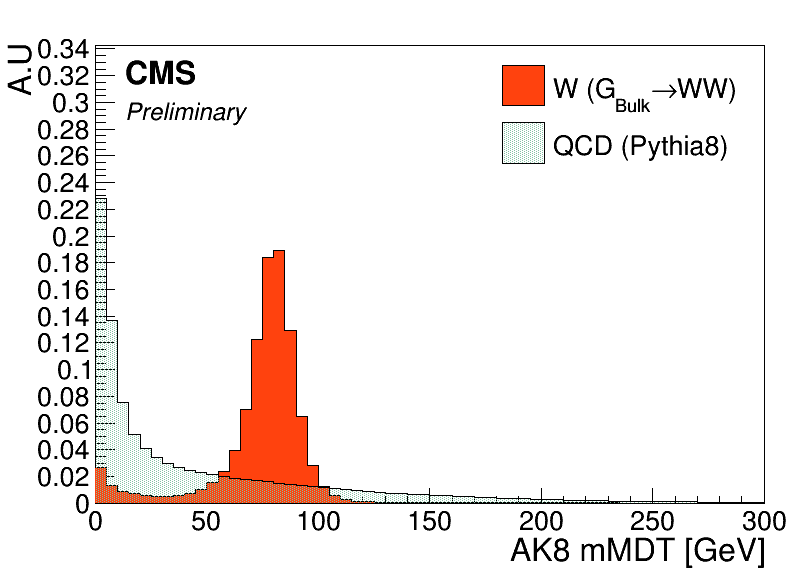
\includegraphics[width=0.49\textwidth]{figures/vtagging/AN-18-099/input/inputs/sig-bkg/msoftdrop_beta0.png}
\caption{Jet \PT (top left), $\eta$ (top right), \nsubj (bottom left) and softdrop jet mass (bottom right) for signal and background jets.}
\label{fig:lola:kinematics}
\end{figure}
The jet \PT distribution is clearly very different between the two samples and, in order to avoid that the network learns jet \PT to be a discriminating feature, we compute a jet-by-jet weight intended to flatten the \PT spectrum during training (making high mass QCD jets and low mass signal jets count more during training). Figure~\ref{fig:lola:ptweight} shows the jet \PT distribution without any \PT-reweighting applied (solid lines) and after applying a \PT-weight (dashed lines). This weight will be used when computing the neural network loss function for a given jet, a process which will be explained further in Section~\ref{sec:lola:training}.
\begin{figure}[h!]
\centering
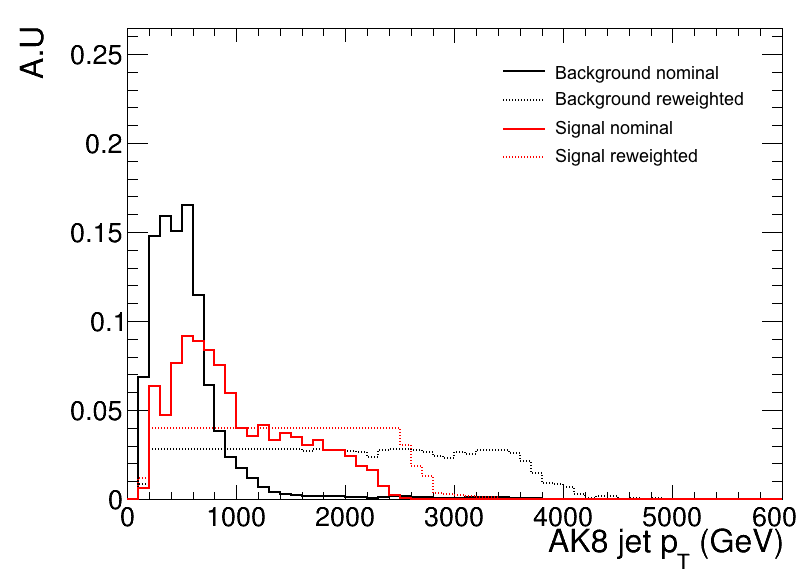
\includegraphics[width=0.49\textwidth]{figures/vtagging/AN-18-099/input/pt_reweighted/postWeight.png}
\caption{Jet \PT distribution before (solid lines) and after (dashed line) applying a weight intended to flatten the jet \PT spectrum.}
\label{fig:lola:ptweight}
\end{figure}
From these signal and background jets, only the jet constituent four vectors of the 20 highest-\PT particles are used as input to the deep neural network: $E$, $p_x$, $p_y$ and $p_z$. I use 20 constituents as any larger number has a negligible affect on the performance, while performance tends to drop once going below 15. The input is therefore a $4 \times N=20$ matrix for each signal and background jet, one four-vector for each of the 20 jet constituents:
\begin{equation}
x_{\mu,i}=\begin{pmatrix}
E^1 & E^2 & \dots & E^N \\[1ex]
p_x^1 & p_x^2 & \dots & p_x^N \\[1ex]
p_y^1 & p_y^1 & \dots & p_y^N \\[1ex]
p_z^1 & p_z^2 & \dots & p_z^N
\end{pmatrix}
\end{equation}
The total number of jet constituents is shown in Figure~\ref{fig:lola:nconst}, and the input variables (here for all constituents) is shown in Figure~\ref{fig:lola:inputs}.\newline
\begin{figure}[h!]
\centering
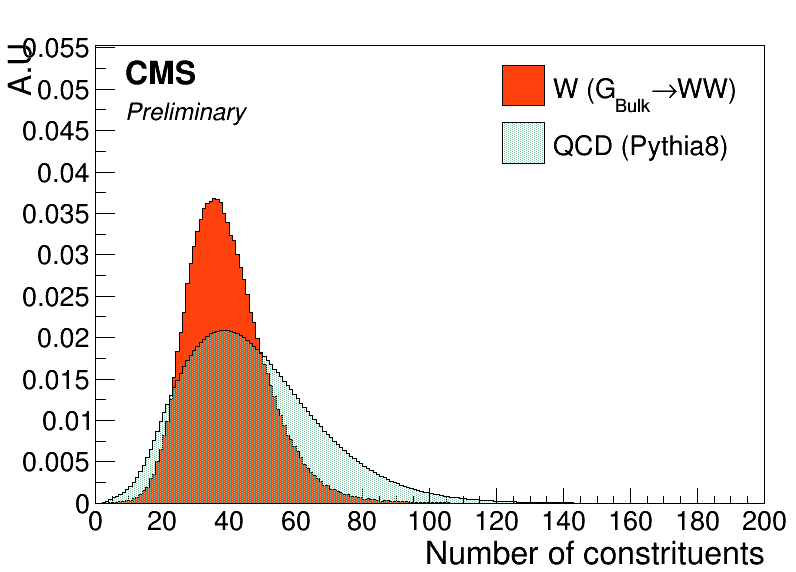
\includegraphics[width=0.49\textwidth]{figures/vtagging/AN-18-099/input/inputs/sig-bkg/nconst.png}
\caption{The number of jet constituents for signal (red) and background (blue). Only the 20 highest-\PT constituents are used during training.}
\label{fig:lola:nconst}
\end{figure}
\begin{figure}[h!]
\centering
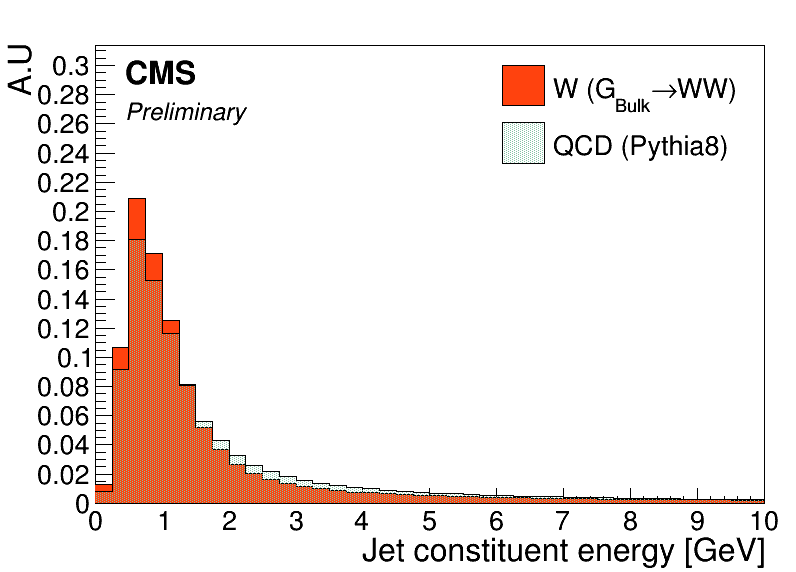
\includegraphics[width=0.49\textwidth]{figures/vtagging/AN-18-099/input/inputs/sig-bkg/pe.png}
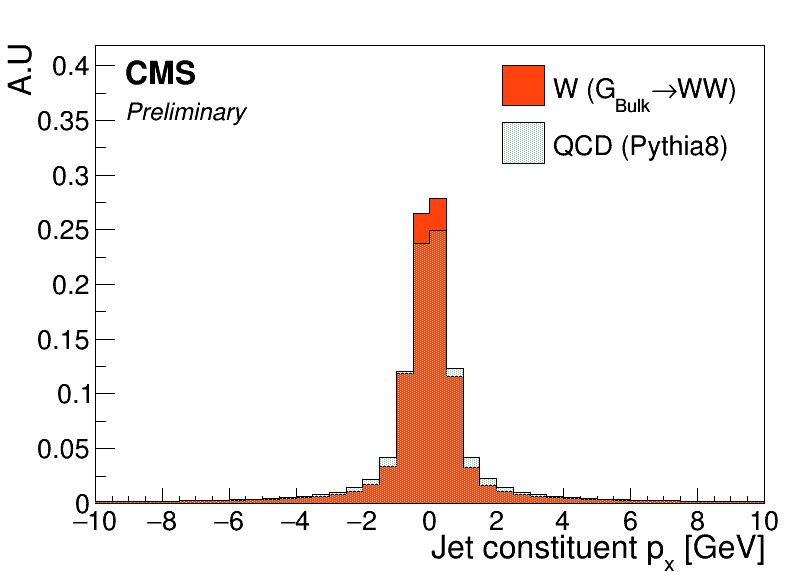
\includegraphics[width=0.49\textwidth]{figures/vtagging/AN-18-099/input/inputs/sig-bkg/ppx.png}\\
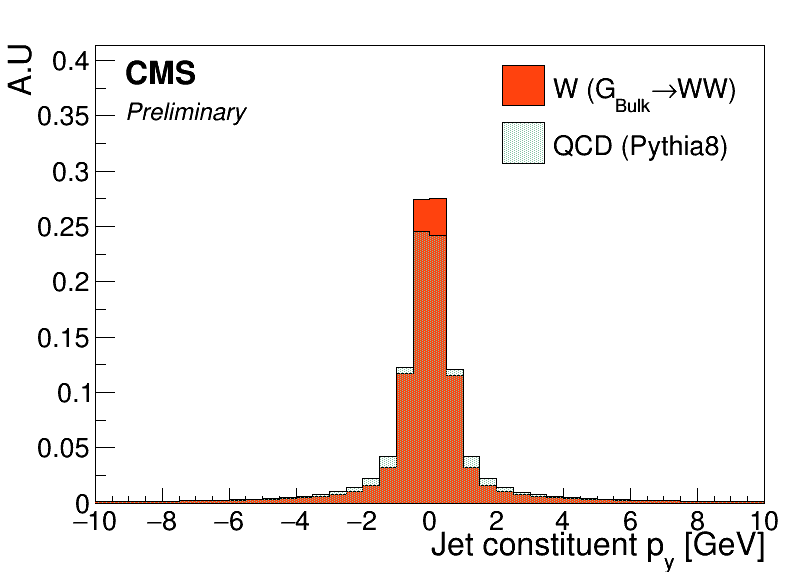
\includegraphics[width=0.49\textwidth]{figures/vtagging/AN-18-099/input/inputs/sig-bkg/ppy.png}
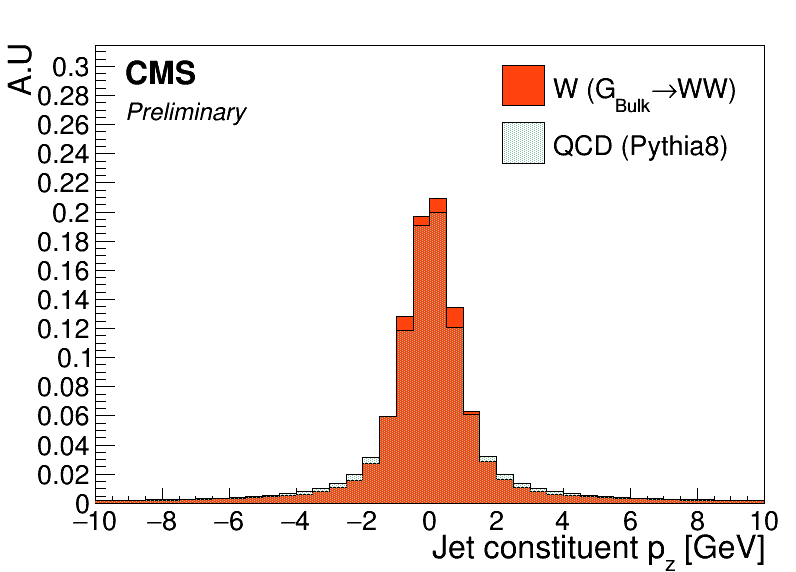
\includegraphics[width=0.49\textwidth]{figures/vtagging/AN-18-099/input/inputs/sig-bkg/ppz.png}
\caption{Energy (top left), $p_x$ (top right), $p_y$ (bottom left) and $p_z$ (bottom right) for all jet constituents. These values are used as input to the neural network training.}
\label{fig:lola:inputs}
\end{figure}
It is clear that the input variables provide little discriminating power on their own. Therefore, the network must learn how to derive other physical quantities where the signal and background PDFs differ to a larger extent. This is achieved through the two custom layers described in the following.

\subsection{The Combination Layer}
\label{sec:cola}
The Combination Layer (CoLa) consists of a matrix which, when takin the scalar product with the input matrix, compute linear combinations of the jet constituents, similar to what is done in recombination jet algorithms. The main goal here is to create additional four-vectors as input for the next layer. The CoLa matrix is a concatenation of the following: A vector of 1's of length $N$, the $N \times N$ identity matrix ($N=20$) and a matrix of $N \times M$ trainable weights.
\begin{equation}
  C_{i,j}=\begin{pmatrix}
1 & 1 & 0 & \dots & 0 & w_{1,N+2} & w_{1,N+3}                & \dots & w_{1,(N+2)+M)} \\
1 & 0 & 1 & \dots & 0 & w_{2,N+2} & w_{2,N+3}                & \dots & w_{2,(N+2)+M)} \\
\vdots & \vdots & \vdots & \ddots & \vdots & \vdots & \vdots & \vdots & \vdots \\
1 & 0 & 0 & 0 & 1 & w_{N,N+2} & w_{N,N+3}                    & \dots & w_{N,(N+2)+M)} 
\end{pmatrix}
\end{equation}
When performing the following multiplication
\begin{equation}
  x_{\mu,i}^{C} = x_{\mu,i}  C_{i,j}
\end{equation}
the resulting output matrix will have dimensions $4 \times (1+N+M)$ and consists of the following: A first column containing the sum of all constituent momenta, the four-momenta of each individual constituent, and M=14 different linear combinations of particles with trainable weights. The first corresponds to the neural network computing the four-vector of the ``full'' jet, at least the full jet in terms of its 20 highest-\PT constituents. The second, simply passes each original constituent four-momentum to the next layer. The final, and most interesting part, lets the network construct alternative subjet four-vectors by letting it weigh constituents up and down as it sees fit in order to reach optimal discrimination power. As an example, lets look at the effect of CoLa in the simple case of only two input jet constituents and two trainable linear combinations:
\begin{equation*}
  \footnotesize
  \begin{centering}
  \begin{pmatrix}
    E^1 & E^2\\[1ex]
    p_x^1 & p_x^2\\[1ex]
    p_y^1 & p_y^1\\[1ex]
    p_z^1 & p_z^2
  \end{pmatrix}
  \begin{pmatrix}
    1 & 1 & 0 & & w_{1,4} & w_{1,5}\\[1ex]
    1 & 0 & 1 & & w_{2,4} & w_{2,5}\\
  \end{pmatrix}
  = \begin{pmatrix}
    E^1  +E^2   & E^1   & E^2   & w_{1,4}E^1   + w_{2,4}E^2   & w_{1,5}E^1  +w_{2,5}E^2    \\[1ex]
    p_x^1+p_x^2 & p_x^1 & p_x^2 & w_{1,4}p_x^1 + w_{2,4}p_x^2 & w_{1,5}p_x^1+w_{2,5}p_x^2  \\[1ex]
    p_y^1+p_y^1 & p_y^1 & p_y^1 & w_{1,4}p_y^1 + w_{2,4}p_y^1 & w_{1,5}p_y^1+w_{2,5}p_y^1  \\[1ex]
    p_z^1+p_z^2 & p_z^1 & p_z^2 & w_{1,4}p_z^1 + w_{2,4}p_z^2 & w_{1,5}p_z^1+w_{2,5}p_z^2
  \end{pmatrix}
   \end{centering}
\end{equation*}
 In the two last columns, the neural network makes two ``subjet'' four-vectors by weighting the relative contribution of each particle as it sees fit. This is similar to jet grooming (Section~\ref{sec:objreco:grooming}) or PUPPI pileup subtraction (Section~\ref{subsub:objreco:puppi}), and should allow the network to learn which constituents are part of the hard scatter and which are not. The $x_{\mu,i}^{C}$ matrix is finally passed on to the next layer, the Lorentz Layer.
\subsection{The Lorentz Layer}
The Lorentz Layer (LoLa) is responsible for encoding how particles move in space-time through a simple set of rules. Each column (four-vector) of $x_{\mu,i}^{C}$, is used to compute, and afterwards is replaced by, the following $k=7$ features:
\begin{equation}
  x_{k,i}^{L} = \begin{pmatrix}
  m^2  (x_{\mu,i}^{C})                       \\[1ex]
  \PT  (x_{\mu,i}^{C})                       \\[1ex]
  w_E E(x_{\mu,i}^{C})                       \\[1ex]
  w^s_1\sum d^2(x_{\mu,i}^{C},x_{\mu,j}^{C}) \\[1ex]
  w^s_2\sum d^2(x_{\mu,i}^{C},x_{\mu,j}^{C}) \\[1ex]
  w^m_1\min d^2(x_{\mu,i}^{C},x_{\mu,j}^{C}) \\[1ex]
  w^m_2\min d^2(x_{\mu,i}^{C},x_{\mu,j}^{C}) 
  \end{pmatrix}
\end{equation}
Going through from top to bottom, these are: The invariant mass of each four-vector, the transverse momentum, the energy together with a trainable weight, the sum of distances between the four-vector under consideration and every other column with two trainable weights and finally the minimum distance between the four-vector under consideration and every other column, also with two trainable weights. The Minkowski metric enters explicitly in the first and in the last four calculations, where the neural network is told to abide by the rules
\begin{equation}
  m^2 (x_{\mu,i}^{C}) = g^{\mu\nu}x_{\mu,i}^{C}x_{\nu,i}^{C}
\end{equation}
and
\begin{equation}
  d^2 (x_{\mu,i}^{C},x_{\mu,j}^{C}) = (x_{\mu,i}^{C}-x_{\mu,j}^{C})_{\mu} g^{\mu\nu} (x_{\mu,i}^{C}-x_{\mu,j}^{C})_{\nu}
\end{equation}
with $g^{\mu,\nu}=[-1,1,1,1]$, when calculating the invariant mass and distance between particles/subjets. This makes the neural network aware of which laws of physics apply when combining four-vectors.  
\section{Decorrelating from mass and $p_{T}$}
\section{Performance}
\section{Model validation}
\label{sec:validation}

The model is validated on independent samples as an unbiased measure of performance. These samples are listed in Table~\ref{tab:validationSamples}.
For these studies we require only hadronically decaying W bosons, where the generated W follows the following criteria:
\begin{itemize}
\item $ 1000 \GeV < \PT < 1400 \GeV$
\item $|\eta| < 1.5$
\item Only use jets where the two W decay products are contained within the jet with $\Delta R < 0.8$
\end{itemize}
For the background, we require the same $\PT$ and $\eta$ cuts as for signal. The signal efficiency versus mistagging rate for LoLa compared to
the standard PUPPI Softdrop + \nsubj tagger, is shown in Figure~\ref{roc_val}. As was pointed out in Section~\ref{sec:training}, a mass cut is not necessary when using LoLa, but have been added to this plot for completeness. A significant improvement in tagging efficiency is observed for LoLa compared to the default tagger. Also marked are the 30 percent signal efficiency working points which are used as reference working points for the following correlation study,


\begin{figure}[htb]
\centering
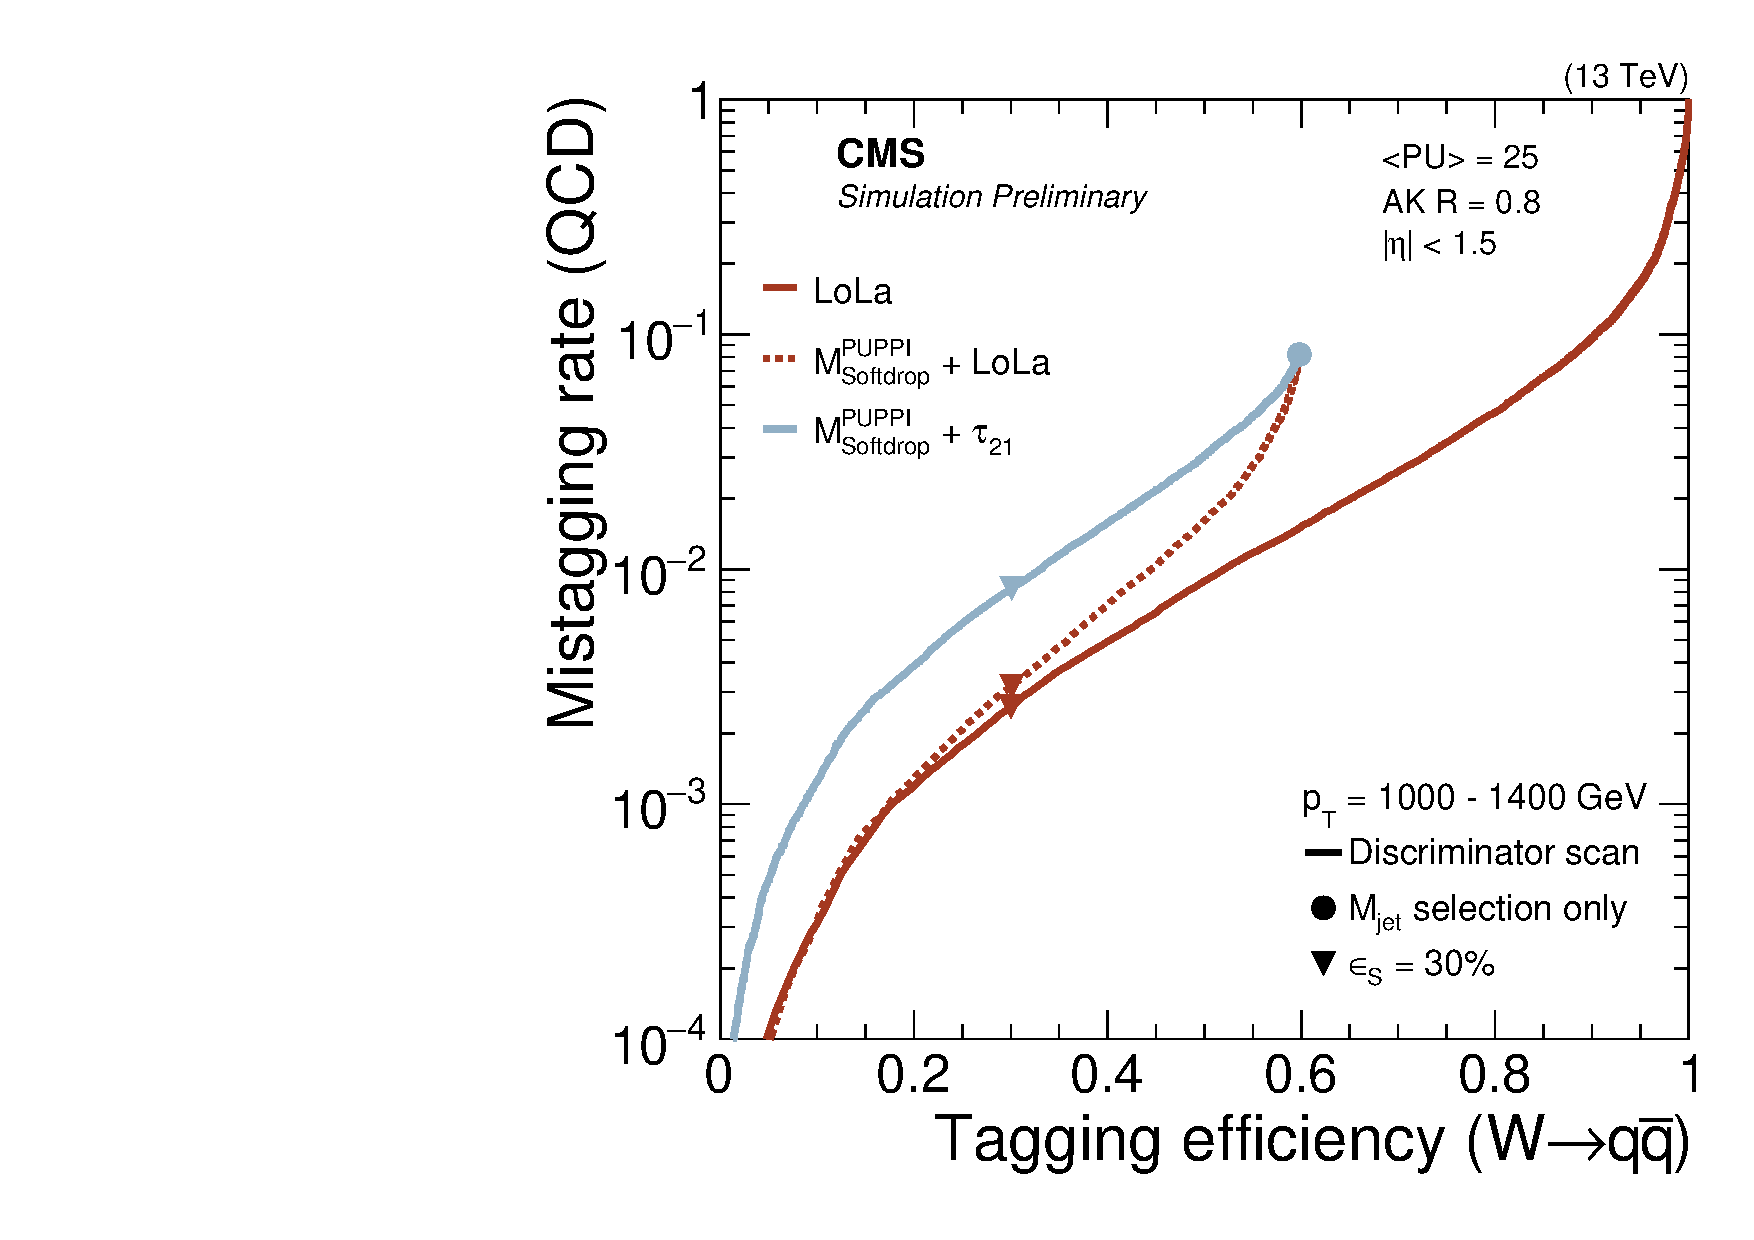
\includegraphics[width=0.49\textwidth]{figures/vtagging/AN-18-099/validation/roc_ZpWqqvsQCD.pdf}\\

\caption{Performance of LoLa and  PUPPI Softdrop + $\tau_{21}$background-signal efficiency plane. The PUPPI softdrop jet mass
selection of $65 < M_{SD} < 105 GeV$, and the 30 percent efficiency points are indicated with symbols.}
\label{fig:roc_val}
\end{figure}


\begin{figure}[htb]
\centering

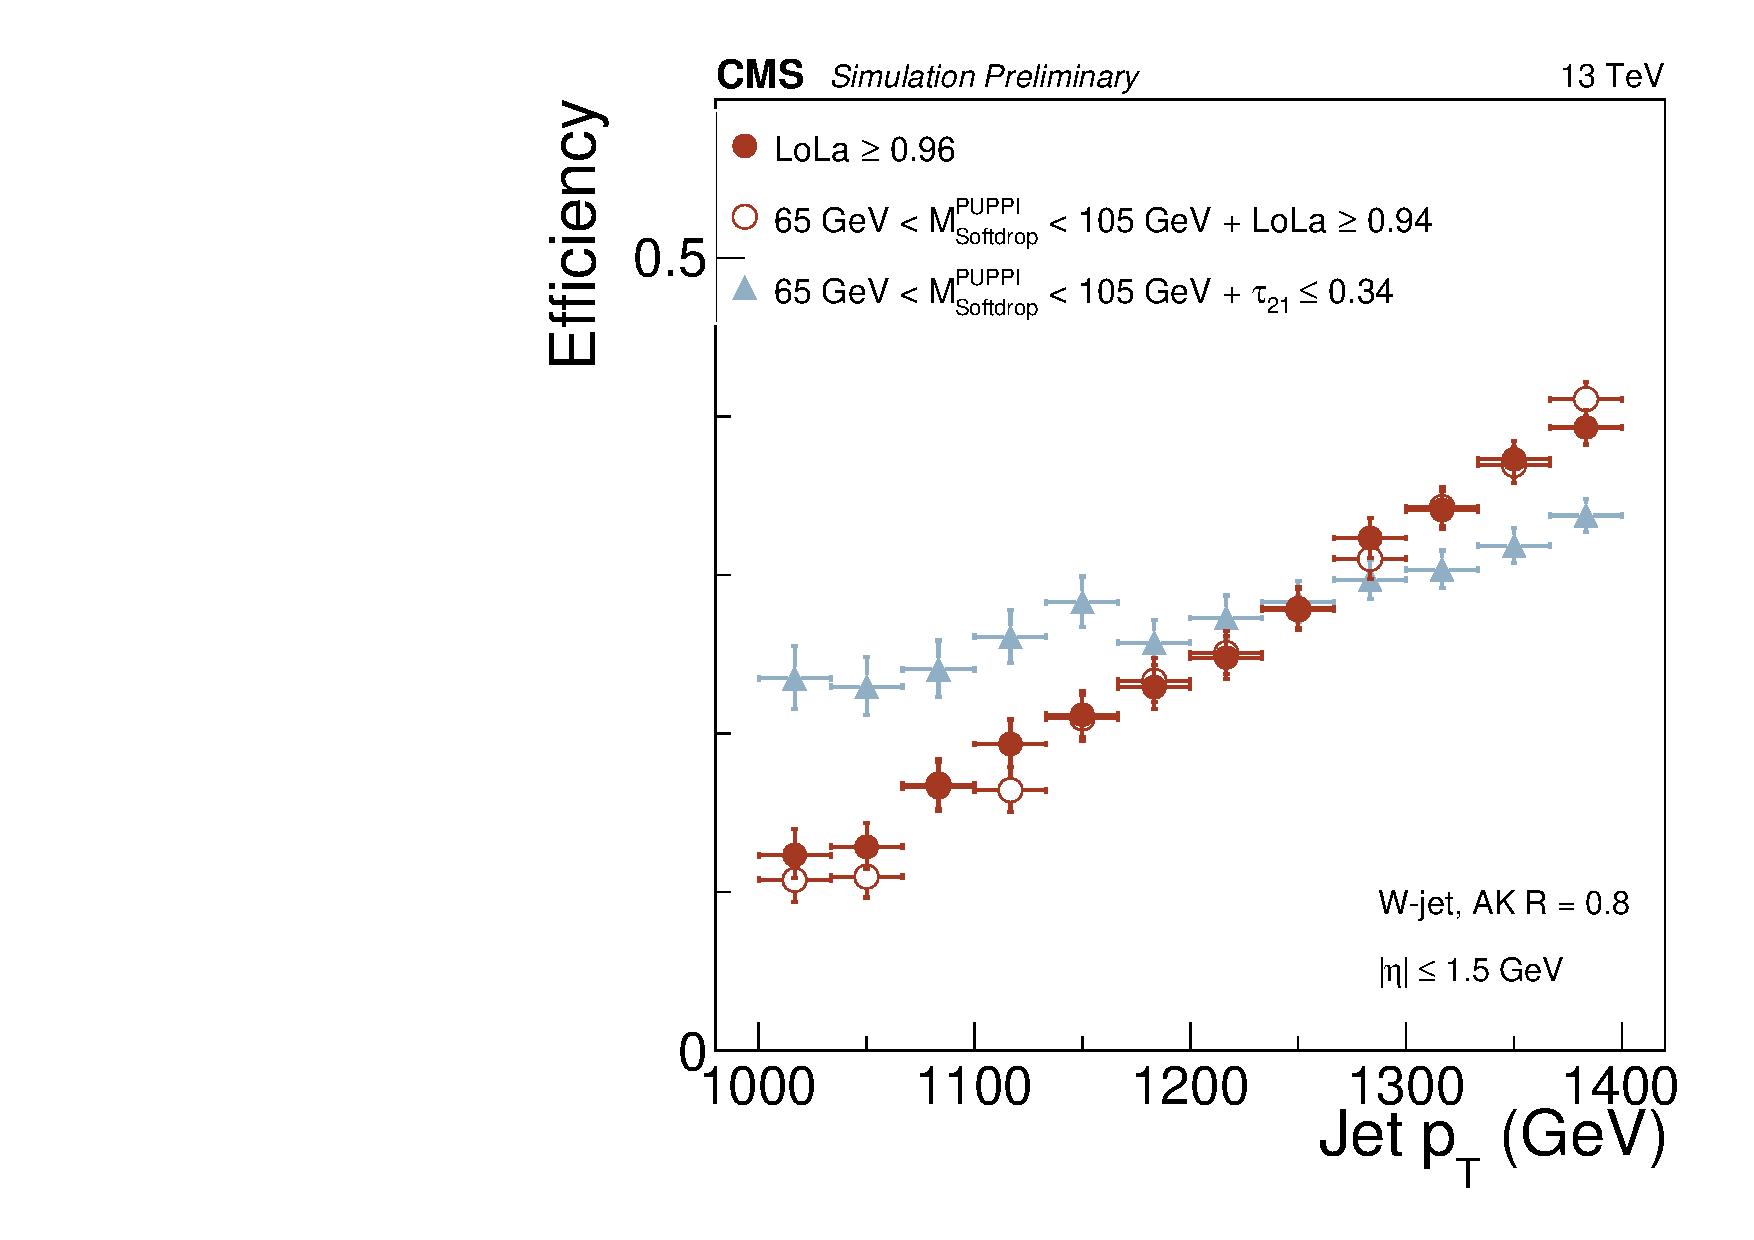
\includegraphics[width=0.49\textwidth]{figures/vtagging/AN-18-099/validation/WtagSigEffvsjpt.pdf}
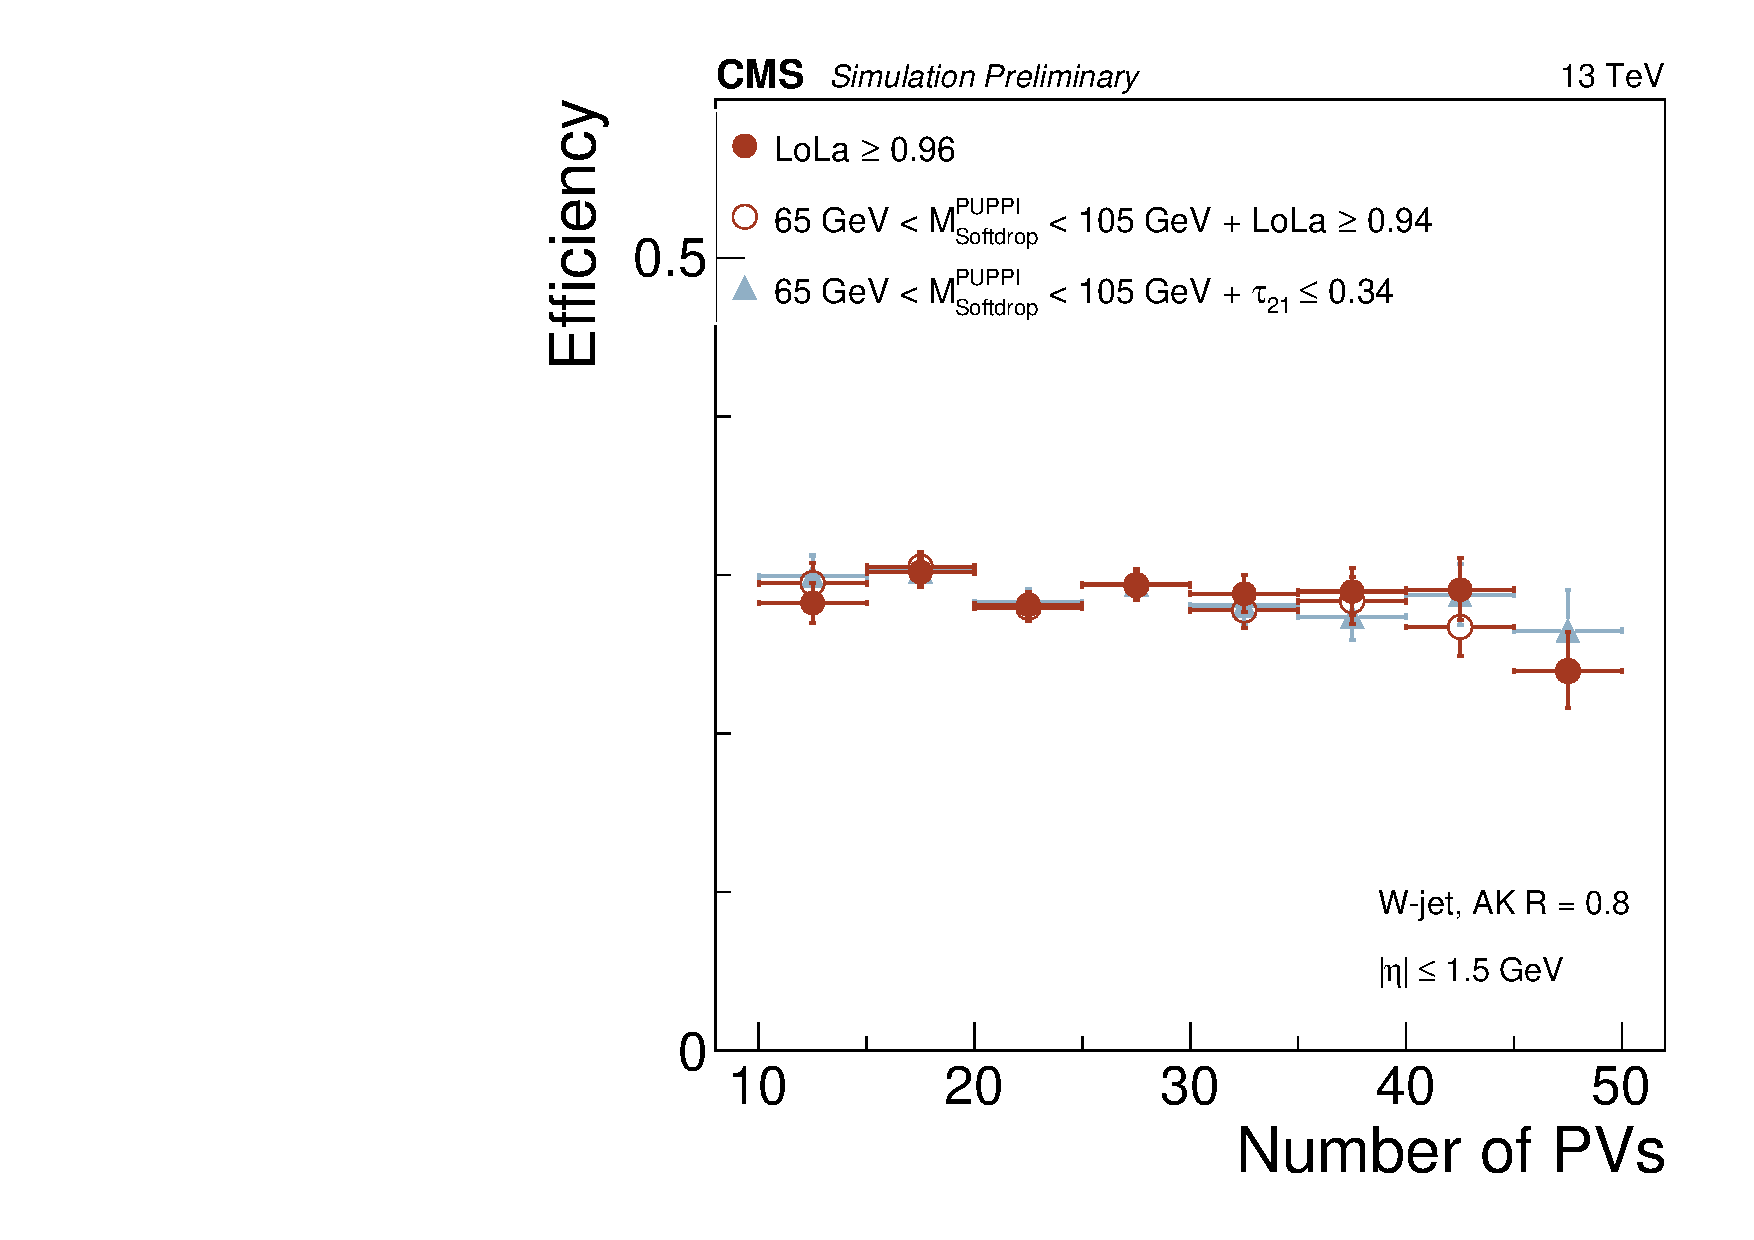
\includegraphics[width=0.49\textwidth]{figures/vtagging/AN-18-099/validation/WtagSigEffvsnPV.pdf}\\
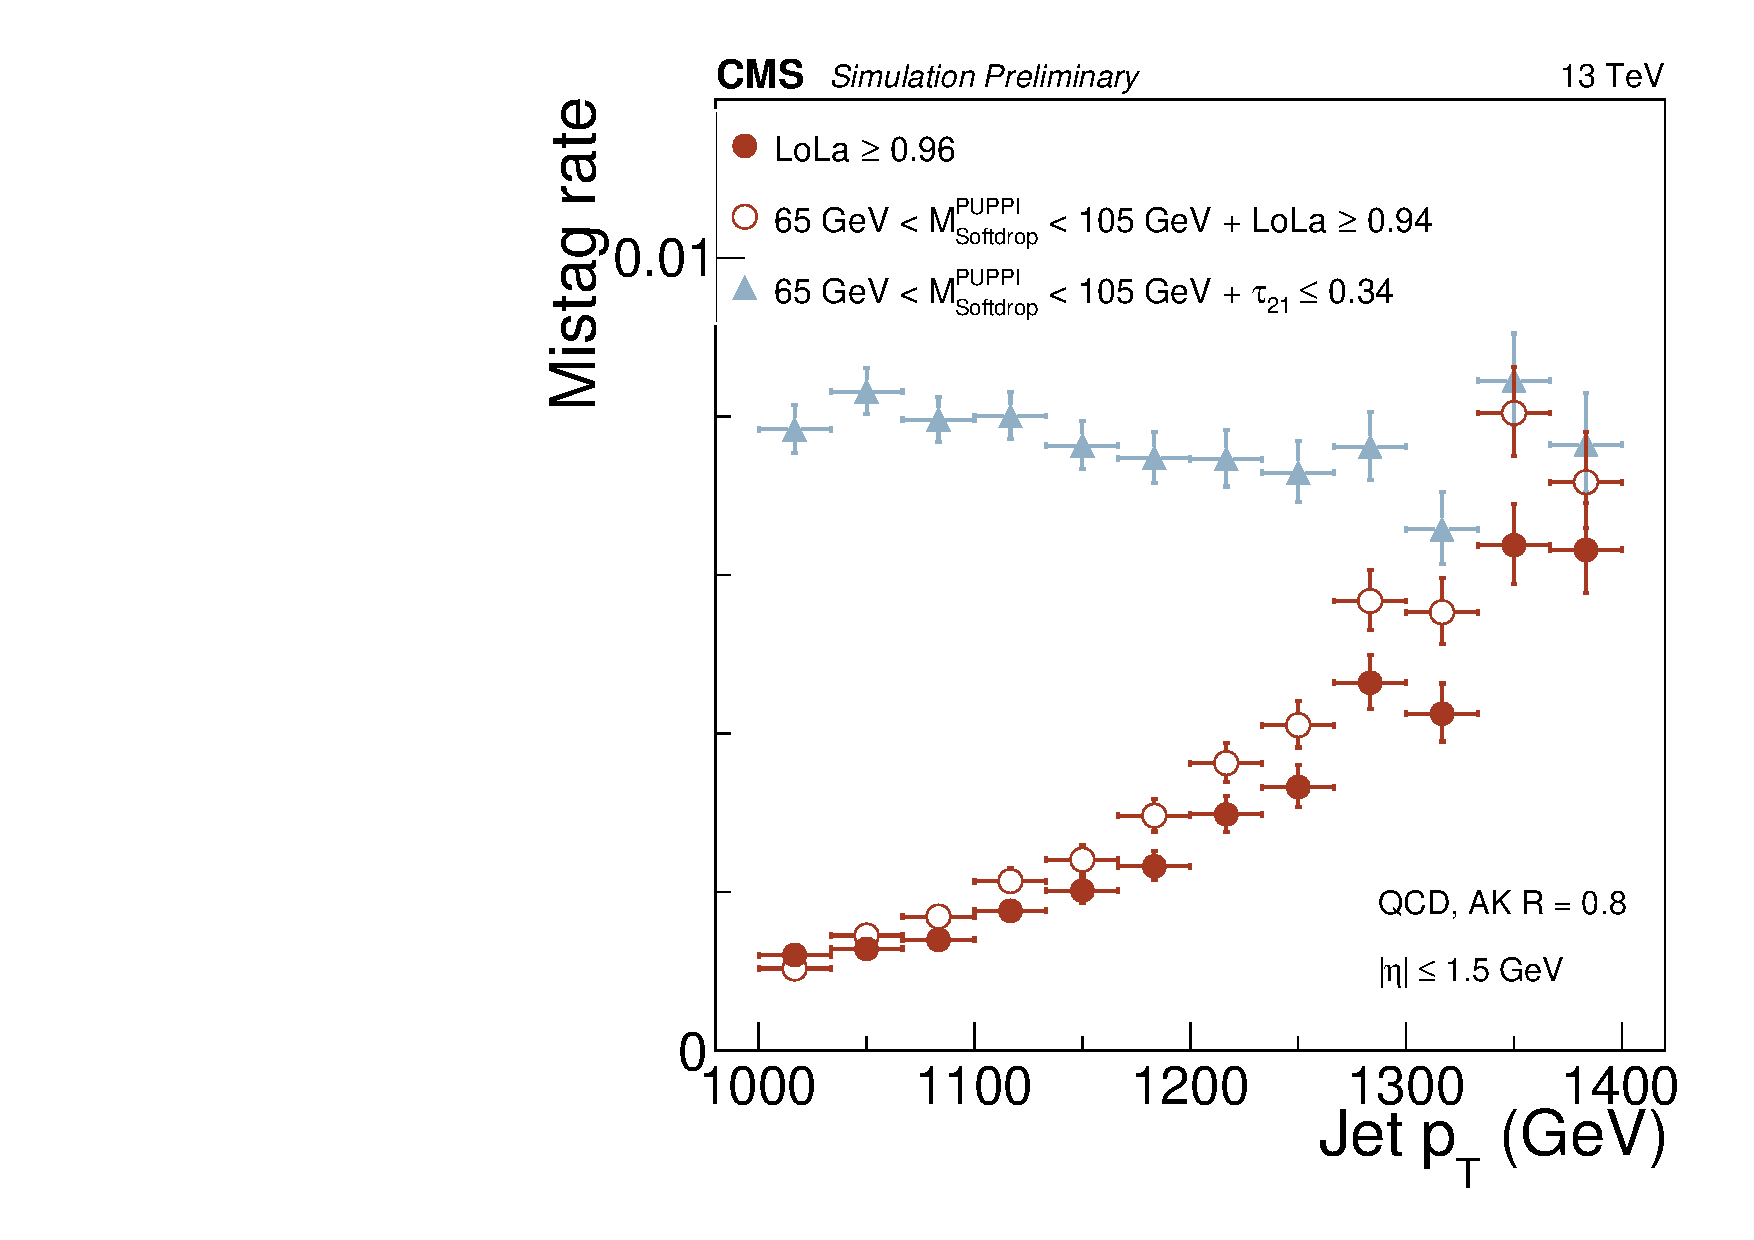
\includegraphics[width=0.49\textwidth]{figures/vtagging/AN-18-099/validation/QCDMistagvsjpt.pdf}
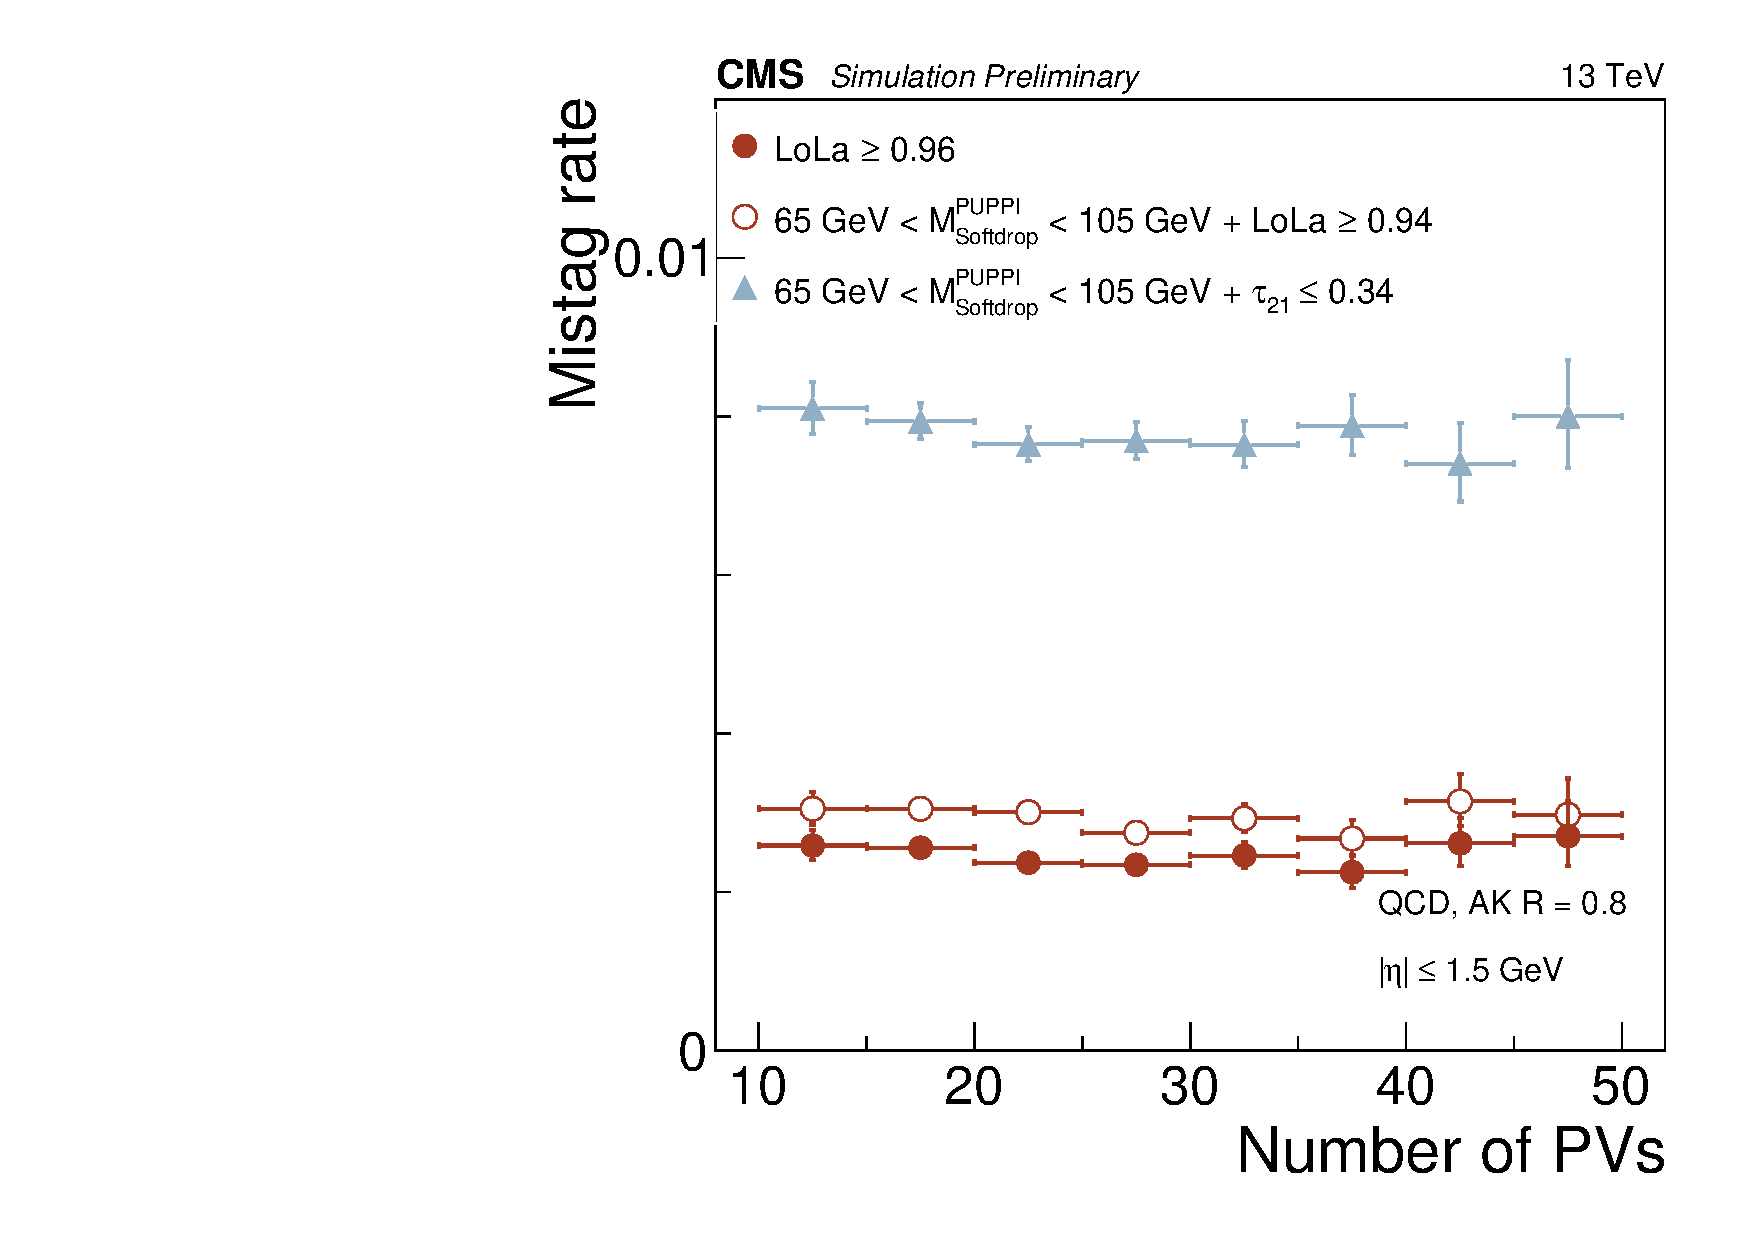
\includegraphics[width=0.49\textwidth]{figures/vtagging/AN-18-099/validation/QCDMistagvsnPV.pdf}


\caption{Top: Efficiency of the LoLa selection corresponding to a 30 percent signal efficiency as a function of (left) \PT and (right) the number of reconstructed vertices. Bottom: Mistag rate of the LoLa selection corresponding to a 30 percent signal efficiency as a function of (left) \PT and (right) the number of reconstructed vertices.}
\label{fig:eff_val}
\end{figure}
\clearpage